\item \points{30}	{\bf Convergence and Learning Rate for Gradient Descent}

When running an optimization algorithm, finding a good learning rate may require some tuning. 
If the learning rate is too high, the gradient descent (GD) algorithm might not converge. If the learning rate is too low, GD may take too long to converge.
In this question, we will investigate some theoretical guarantees for the convergence of GD on convex objective functions, and their implications on choosing the learning rate.

{\bf Recap and notation.} Suppose we have a convex
objective function $J(\theta)$. At each iteration, GD updates the iterate $\theta^{[t]}$ as 
follows:
\begin{equation*}
	\theta^{[t]} = \theta^{[t-1]} - \alpha\nabla J(\theta^{[t-1]})
\end{equation*}

where $\alpha$ is the learning rate and $\nabla J(\theta^{[t-1]})$ is the gradient of $J(\theta)$ evaluated at $\theta^{[t-1]}$.

\begin{enumerate}
\item \points{8} {\bf Quadratic Objective, Scalar Variable}

In this part, consider the simple objective function with one-dimensional variable $\theta$:
\begin{equation*}
	J(\theta) = \frac{1}{2}\beta\theta^2
\end{equation*}
where $\theta \in\mathbb{R}$ is our parameter and $\beta\ > 0$ is a positive, constant scalar.
We initialize GD at some initialization $\theta^{[0]} \neq 0$ and run GD with learning rate $\alpha$. 

\begin{enumerate}
	\item \textbf{Derive} the range of $\alpha$ such that the iterate of GD converges in the sense that there exists a scalar $\theta^\dagger$ such that $\lim_{t\to\infty} |\theta^{[t]}-\theta^\dagger| = 0$.   Provide the value of $\theta^\dagger$ when GD converges and show that it's equal to the global minimum $\theta^* = \arg\min_\theta J(\theta)$. The range of $\alpha$ can potentially depend on $\beta$. 
	\item Given a desired accuracy $\epsilon > 0$, for all the $\alpha$ in the range that you derived, \textbf{derive} the minimum number of iterations $T$ required to reach a point $\theta^{[T]}$ such that $|\theta^{[T]} - \theta^*| \le \epsilon$. $T$ can potentially depend on $\epsilon$, $\theta^{[0]}$, $\alpha$, and $\beta$. Investigate the behavior of $T$ and whether $T$ is increasing or decreasing for different values of $\alpha$. Briefly discuss why choosing an inappropriate $\alpha$ can cause the algorithm to take longer to converge.
\end{enumerate}

\textit{Hint:} Express $\theta^{[t]}$ in terms of $\theta^{[0]}$, $\alpha$, $t$, and $\beta$. 

\textit{Hint:} $\lim_{t\to\infty} c^t = 0, \quad\forall c\in\mathbb{R} \ s.t.\ |c|<1$ 


\ifnum\solutions=1{
  \begin{answer}
\newpage
\end{answer}

}\fi

\item \points{4} {\bf Quadratic Objective, d-dimensional Variable}

In this part of the question, consider the objective function with $d$-dimensional variable $\theta$:
\begin{equation*}
	J(\theta) = \frac{1}{2}\sum_{i=1}^d \beta_i\theta_i^2
\end{equation*}
where $\theta_i$'s are our parameters and $\beta_i\in \mathbb{R}\ s.t.\ \beta_i > 0$ are positive, constant scalars.
Assume that we start from some $\theta^{[0]}$\ where	$\theta_i^{[0]} \neq 0$ for all $i$ and run GD with learning rate $\alpha$. Derive the range of learning rate $\alpha$ such that GD converges in the sense that there exists a vector $\theta^\dagger\in \mathbb{R}^d$ such that $\lim_{t\to\infty} \|\theta^{[t]}-\theta^\dagger\|_2 = 0$.   Provide the value of $\theta^\dagger$ when GD converges. The range of $\alpha$ can potentially depend on $\beta_i$ where $i \in \{1,\dots,d\}$. 


\ifnum\solutions=1{
	\begin{answer}
\newpage
\end{answer}
}\fi

\item \points{4} {\bf Coding Question: Quadratic Multivariate Objective}

Let the objective function be 
\begin{equation*}
	J(\theta) = \theta^\top A\theta
\end{equation*}

where $A\in\mathbb{R}^{2\times 2}$ is a $2 \times 2$ real, positive semi-definite matrix. Do the following exercises:

\begin{enumerate}
	\item Implement the \texttt{update\_theta} and \texttt{gradient\_descend} function in \url{src/gd_convergence/experiment.py}. You can stop the GD algorithm when either of the following condition is satisfied:
	\begin{enumerate}
		\item $|J(\theta^{[t]}) - J(\theta^{[t-1]})| < \epsilon$ where $\epsilon=10^{-50}$ is given as the function parameter. This is when we assume the algorithm converged. 
		\item $J(\theta^{[t]}) > 10^{20}$. This is to prevent an infinite loop when the algorithm does not converge.
	\end{enumerate}
	To test your implementation, run \texttt{python src/gd\_convergence/experiment.py}, which checks that your $\theta$ (approximately) converges to the optimal value. \\
	\\
	Note that we have provided you a matrix $A=\begin{bmatrix} 1 & 0 \\ 0 & 2 \end{bmatrix}$ and $\theta^{[0]} = [-1, 0.5]$ at the beginning of the file for you to experiment with. Therefore, the objective function is a special case of the objective function in part (b) with dimension $d=2$. Check if your theoretical derivation of the feasible range of the learning rate indeed matches empirical observations. 
	\item Now, suppose we rotate the matrix $A$, what do we observe?
	 Plot the trajectories of the GD algorithm using the following learning rates: $0.05$, $0.1$, $0.2$, $0.3$, $0.4$, $0.45$, $0.5$, and $1$. We have provided the rotation and plotting function for you. You need to simply run \texttt{python src/gd\_convergence/plotting.py lr1 lr2 lr3 ...} with \texttt{lr*} replaced with desired learning rates. Include the output file \url{trajectories.png} and \url{trajectories_rotated.png}, as well as a brief discussion on the printed output of \url{plotting.py} in the write-up. 

     \smallskip

     \emph{Remark: } If you find that a learning rate of $0.5$ is resulting in non-terminating behavior, this may be due to numerical instability. In this case, feel free to use a learning rate of $0.55$ in place of $0.5$. 
\end{enumerate}

Note that setting the learning rate too high will cause the objective function to not converge. The convergence properties of these learning rates are also rotational invariant. We will show this formally in the next part of the problem.

\ifnum\solutions=1{
	\begin{answer}
\newpage
Following is the printed output of the program. 
\begin{figure}[H]
  \centering
  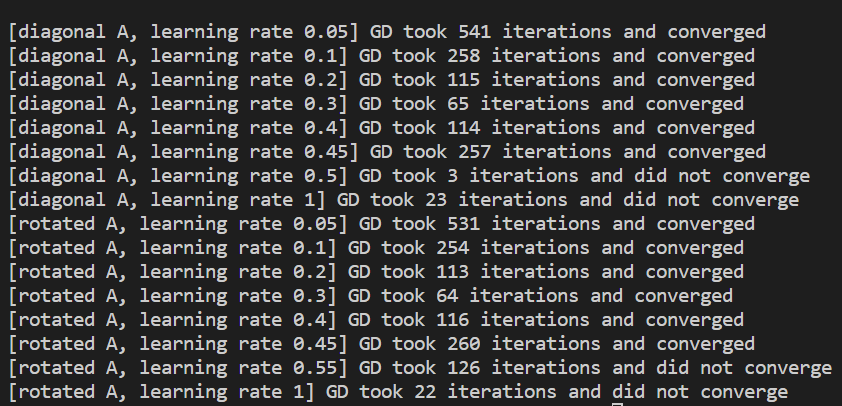
\includegraphics[width=0.9\textwidth]{gd_convergence/conv_rate_gd.PNG}
\end{figure}
We have that $\nabla J(\theta) = 2A\theta$, and therefore $\theta^{[t]} = (I-2\alpha A)^t\theta^{[0]}$. Thus by (b), GD converges if $0<\alpha<\frac{1}{A_{ii}}$, for all $i$.
From the output we see that GD converges for learning rate up until $\alpha = 0.5$, $max(A_{ii})=2$ so that matches the theoretical value. We also observe that the convergence is much slower for values close to the bounds, $(0, 0.5)$
\begin{figure}[H]
  \centering
  \begin{subfigure}[b]{0.49\textwidth}
    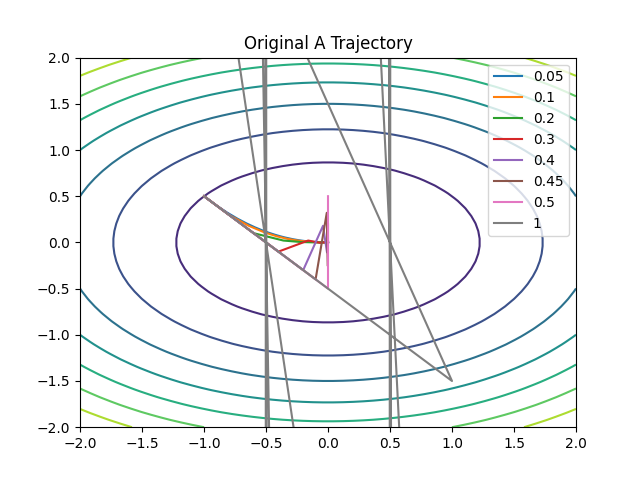
\includegraphics[width=\textwidth]{gd_convergence/trajectories.png}
  \end{subfigure}
  \begin{subfigure}[b]{0.49\textwidth}
    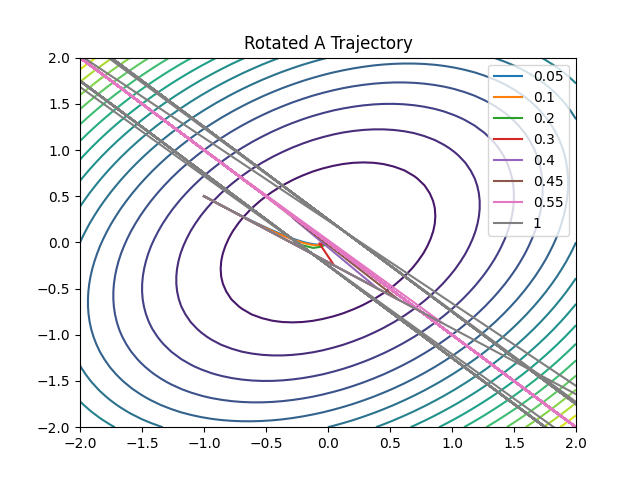
\includegraphics[width=\textwidth]{gd_convergence/trajectories_rotated.png}
  \end{subfigure}
\end{figure}
\newpage
\end{answer}
}\fi

\item \points{12} {\bf Convergence of Gradient Descent for a General Convex Objective}

Now let's consider any convex, twice continuously differentiable objective function $J(\theta)$ that is bounded from below.
Suppose that the largest eigenvalue of the Hessian matrix $H=\nabla^2 J(\theta) $ is less than or equal to $\beta_{\max}$ for all points $\theta$.


Show that when running gradient descent, choosing a step size $0 < \alpha < \frac{1}{\beta_{\max}}$ guarantees that $J(\theta^{[t]})$ will converge to some finite value as $t$ approaches infinity.\footnote{This definition of convergence is different from the definition in previous questions where we explicitly prove that the parameter $\theta$ converges to an optimal parameter $\theta^*$. In this case, we do not know the optimal value $\theta^*$, and it would be difficult to prove convergence using the previous definition.} Specifically, you should derive an inequality for $J(\theta^{[t]})$ in terms of $J(\theta^{[t-1]})$, $\nabla J(\theta^{[t-1]})$, $\alpha$, and $\beta_{\max}$, and show that the objective function is strictly decreasing during each iteration, i.e. $J(\theta^{[t]}) < J(\theta^{[t-1]})$.


\textit{Hint:} You can assume that, by Taylor's theorem, the following statement is true:
\begin{equation*}
	J(y) = J(x) + \nabla J(x)^\top (y-x) + \frac{1}{2}(y-x)^\top \nabla^2 J(x + c(y-x)) (y-x) \text{ for some } 0 \leq c \leq 1
\end{equation*}


\textit{Hint:} The Hessian of a convex function is symmetric and positive semi-definite at any point $\theta$, which means all of its eigenvalues are real and non-negative.

\textit{Hint:} The Hessian matrix is symmetric. Consider using the spectral theorem introduced in problem 3 in homework 0.

\textit{\textbf{Optional (no credit):}}  Using the gradient descent inequality that you derived, show that the GD algorithm converges in the sense that  $\lim_{t\to\infty}||\nabla J(\theta^{[t]})||_{2}^{2}=0$.\footnote{Note that $\lim_{t\to\infty}||\nabla J(\theta^{[t]})||_{2}^{2}=0$ does not necessarily mean that there exists a vector $\hat{\theta}$ such that $\theta^{[t]} \rightarrow \hat{\theta}$. (Even an 1-dimensional counterexample exists.) However, for convex functions, when $\theta^{[t]}$ stays in a bounded set, $\lim_{t\to\infty}||\nabla J(\theta^{[t]})||_{2}^{2}=0$ does imply that $J(\theta^{[t]}) \rightarrow \inf_\theta J(\theta)$ as $t\rightarrow \infty$. Therefore, $\lim_{t\to\infty}||\nabla J(\theta^{[t]})||_{2}^{2}=0$ is typically considered a reasonable definition for an optimization algorithm's convergence.}

\textit{Remark:} This question suggests that a smaller learning rate should be applied if we believe the curvature of the objective function is big.

\ifnum\solutions=1{
	\begin{answer}
\newpage
\end{answer}

}\fi

\item \points{2} {\bf Learning Rate for Linear Regression}

Consider using GD on the LMS objective introduced in lecture:
\begin{equation*}
	J(\theta) = \frac{1}{2}||X\theta - y||_2^2
\end{equation*}
where $X\in\mathbb{R}^{n\times d}$ is the design matrix of our data, $\theta\in\mathbb{R}^d$ is our parameter, and $\vec{y}\in\mathbb{R}^n$  is the response variable. 

Let $\beta_{\max}$ be the largest eigenvalue of $X^\top X$. Prove that for all  $\alpha \in (0, \frac{1}{\beta_{\max}})$, GD with learning rate $\alpha$ satisfies that $J(\theta^{[t]})$ converges as $t\rightarrow \infty.$
	
\textit{Hint:}	You can invoke the statements in the part (d) (including the optional question in part (d)) to solve this part (even if you were not able to prove part (d).)

\textbf{Remark:} The conclusion here suggests that for linear regression, roughly speaking, you should use smaller learning rates if the scale of your data $X$ is big or if the data points are correlated with each other, both of which will enable a large top eigenvalue of $X^\top X$.

\textbf{Remark:} Even though in many cases the LMS objective can be solved 
exactly by solving the normal equation as shown in lecture, it is still useful to be able to guarantee convergence
when using the Gradient Descent algorithm in situations where it is difficult to solve
for the optimal $\theta^*$ directly (such as having large amount of data making inverting $X$
very expensive).


\ifnum\solutions=1{
	\begin{answer}
\end{answer}

}\fi



\end{enumerate}